\documentclass[10pt,twocolumn]{article}

\usepackage[utf8]{inputenc}
\usepackage[T1]{fontenc}
\usepackage[margin=0.54in, top=0.50in, bottom=0.52in]{geometry}
\usepackage{mathptmx}
\linespread{0.965}
\usepackage{microtype}
\usepackage{amsmath,amssymb}
\usepackage{graphicx}
\usepackage{booktabs}
\usepackage{array}
\usepackage{multirow}
\usepackage{xcolor}
\usepackage{hyperref}
\usepackage{caption}
\usepackage{subcaption}
\usepackage{enumitem}
\usepackage{titlesec}

\hypersetup{
    colorlinks=true,
    linkcolor=blue!60!black,
    citecolor=green!50!black,
    urlcolor=blue!70!black
}

\captionsetup{font=footnotesize, labelfont=bf, skip=3pt}
\setlist[itemize]{noitemsep, topsep=2pt, leftmargin=1.3em}
\setlist[enumerate]{noitemsep, topsep=2pt, leftmargin=1.4em}

\titlespacing*{\section}{0pt}{1.0ex plus 0.2ex minus .1ex}{0.4ex plus .1ex}
\titlespacing*{\subsection}{0pt}{0.7ex plus 0.2ex minus .1ex}{0.3ex plus .1ex}

\setlength{\textfloatsep}{4pt plus 1pt minus 1pt}
\setlength{\floatsep}{4pt plus 1pt minus 1pt}
\setlength{\intextsep}{4pt plus 1pt minus 1pt}

\let\oldthebibliography\thebibliography
\renewcommand{\thebibliography}[1]{%
  \oldthebibliography{#1}%
  \setlength{\itemsep}{0pt}%
  \setlength{\parskip}{0pt}%
}

\title{\vspace{-1.5em}\Large\textbf{ASCIIgent: Agentic ASCII Art Generation}\vspace{-0.4em}}

\author{
  \normalsize Hana Hasan \qquad Amit Arad \qquad Roei Levi \qquad Tom Shur \\[0.2em]
  \small\href{https://github.com/HanaHasan04/asciigent}{\texttt{https://github.com/HanaHasan04/asciigent}}
}
\date{\vspace{-1.6em}}

\begin{document}

\maketitle

\begin{abstract}
\noindent
Visual abstraction is the process of discarding redundant low-level visual data---textures, photometrics, and uninformative pixel noise---and re-encoding semantic structures into a reduced, symbolic visual language. While recent advances in neural sketch synthesis like SketchAgent demonstrate that vision-language models (VLMs) can synthesize continuous vector strokes, we investigate whether this spatial capacity extends to a fundamentally more constrained and discrete medium: \textbf{ASCII art}. In ASCII art, a model must convey recognizable silhouettes using printable characters on a fixed-size monospace character grid. Characters here serve a dual role: simultaneously functioning as language tokens and spatial micro-primitives. This dichotomy introduces a core question: do autoregressive models draw through spatial reasoning or pure textual memorization, and does active visual perception enable meaningful self-correction? We introduce \textbf{ASCIIgent}, a training-free framework evaluating monolithic prompting baselines, agentic discrete tool-use loops, and multimodal visual feedback across Gemini family models (\texttt{gemini-3-flash-preview} and \texttt{gemini-3.1-flash-lite}). Evaluating against structure-destroying scrambled controls to mitigate the text-reading bias of VLM judges, we reveal characteristic failure modes of monolithic generation (scanline drift, glyph collapse, and plan-truncation leakage) and show that iterative visual feedback enables grounded spatial refinement, localized editing, and frame-consistent animation.
\end{abstract}

% =========================================================
\section{Introduction and Related Work}
% =========================================================

\textbf{Visual Abstraction and Agentic Sketching.}
Visual abstraction is a foundational capability of biological and computational perception~\cite{hertzmann2020line}. Neural stroke models pioneered recurrent drawing representations~\cite{ha2017neural}, later advancing toward semantic vector sketching~\cite{vinker2022clipasso}. Recently, \textbf{SketchAgent}~\cite{vinker2025sketchagent} formalized sketch generation as a continuous perception--reasoning--action loop: a frozen multimodal LLM iteratively emits B\'{e}zier stroke control points, inspects the updated rasterized canvas, and refines the drawing. Concurrently, \textbf{VideoSketcher}~\cite{ren2025videosketcher} demonstrated that dynamic sketching can be decomposed into an LLM-guided structural plan coupled with video diffusion priors. We adapt and generalize this agentic paradigm to discrete character media.

\textbf{The ASCII Art Medium and its Challenges.}
ASCII art imposes a strict spatial constraint: characters must occupy fixed coordinates in a monospace grid $\Sigma^{H \times W}$. Unlike continuous splines, characters possess fixed discrete geometry: a forward slash \texttt{/} acts as a $45^\circ$ line segment, an at-sign \texttt{@} acts as a dense tonal patch, and a period \texttt{.} functions as point stippling. Monolithic autoregressive generation suffers from \textbf{scanline drift}: generating left-to-right, top-to-bottom forces the model to commit to features in early rows that must align with geometry hundreds of tokens later without visual verification or backtracking. Public archives like \texttt{asciiart.eu}~\cite{asciiart_archive} document decades of human designs that language models have partially memorized during pretraining.

\textbf{The VLM Evaluation Confound.}
Evaluating ASCII art with multimodal models introduces a severe confounding factor: as shown by Wang et al.~\cite{wang2025textspeaks} and ASCIIBench~\cite{luo2025asciibench}, VLMs systematically suffer from text bias, recognizing concepts by reading character sequences rather than perceiving geometric shapes. Our evaluation incorporates structure-destroying scrambled controls (\emph{scramble-cells} and \emph{scramble-ink}) to isolate genuine visual recognizability.

% =========================================================
\section{Methodology}
% =========================================================

\subsection{Canvas Representation and Format Contract}
We define the drawing canvas as a fixed character matrix $C \in \Sigma^{H \times W}$ with $H=24$ rows, $W=48$ columns, and printable ASCII alphabet $|\Sigma|=95$ (codepoints 32--126). Deterministic monospace rasterization $\mathcal{R}: \Sigma^{24 \times 48} \to \mathbb{R}^{H' \times W' \times 3}$ renders glyphs at exact cell offsets without font kerning. Every model response is validated by a strict parser: row/column overflows or missing code fences are repaired and logged in a \texttt{ParseReport}.

\begin{figure*}[!t]
  \centering
  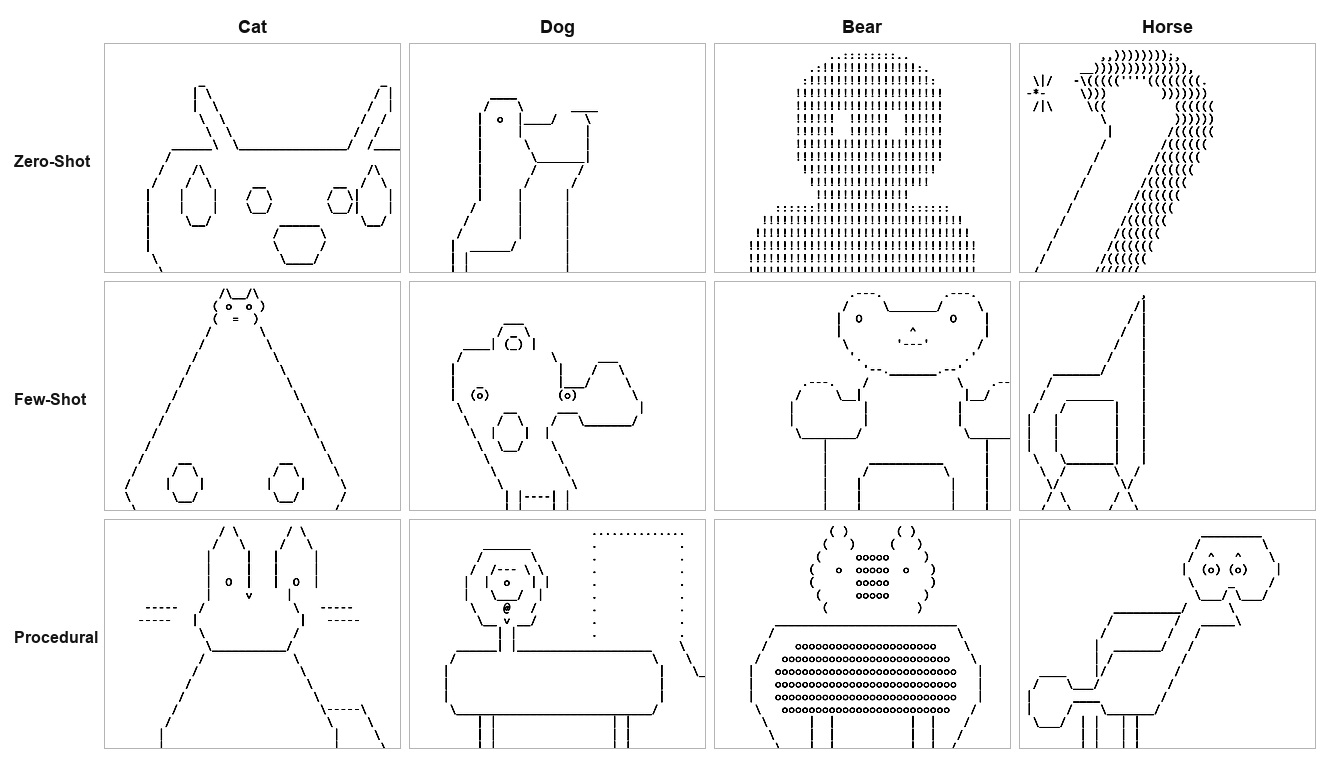
\includegraphics[width=0.88\linewidth, height=3.75cm, keepaspectratio]{figures/p1_contact_sheet.png}
  \vspace{-4pt}
  \caption{\textbf{P1 One-Shot Baseline Contact Sheet (12 Cells, Model: \texttt{gemini-3-flash-preview}).} Columns show the four target categories (\texttt{cat}, \texttt{dog}, \texttt{bear}, \texttt{horse}); rows show the three prompting arms. Zero-shot produces recognizable silhouettes but occasionally drifts across the 48-column right boundary (e.g., \texttt{horse}); few-shot regularizes scale and centering; procedural CoT (with bounded thinking effort \texttt{--effort low}) yields rich anatomical structure such as paws, manes, and hooves.}
  \label{fig:contact_sheet}
\end{figure*}

\subsection{One-Shot Generation Baselines (P1)}
We evaluate three one-shot prompting strategies across four target categories (\texttt{cat}, \texttt{dog}, \texttt{bear}, \texttt{horse}) and two Gemini family models (\texttt{gemini-3-flash-preview} and \texttt{gemini-3.1-flash-lite}):
\begin{enumerate}
  \item \textbf{Zero-Shot:} Direct instruction: ``Draw a \{category\} on the $24 \times 48$ canvas.''
  \item \textbf{Few-Shot:} Same prompt preceded by four hand-crafted exemplar categories (\texttt{fish}, \texttt{house}, \texttt{tree}, \texttt{sailboat}) strictly disjoint from test categories to prevent direct template copying.
  \item \textbf{Procedural (CoT):} The model writes a structured 3-step spatial plan (major parts, row/column bounding regions, and contour glyph choices) before emitting the fenced $24 \times 48$ grid.
\end{enumerate}

\subsection{Agentic Loop and Turn Protocol (P2)}
Instead of emitting all $24 \times 48$ characters monolithically, ASCIIgent interacts with an \texttt{AsciiCanvas} over a multi-turn loop with a budget of $T_{\max} = 3$ turns. In each turn $t \in \{1, 2, 3\}$, the agent emits a JSON batch of multiple discrete tool calls:
\begin{itemize}
  \item \texttt{patch\_edit}$(r, c, \textit{lines})$: Localized subgrid overwrite at 0-indexed $(r, c)$ where alignment spaces preserve underlying ink.
  \item \texttt{draw\_line}$(r_1, c_1, r_2, c_2, \textit{char})$ \& \texttt{draw\_rect}$(t, l, b, r, \textit{border}, \textit{fill})$: Bresenham line and box primitives.
  \item \texttt{shade\_density}$(t, l, b, r, \ell)$ \& \texttt{erase\_rect}$(t, l, b, r)$: Tonal fill (\texttt{' '} $<$ \texttt{'.'} $<$ \texttt{':'} $<$ \texttt{'-'} $<$ \texttt{'='} $<$ \texttt{'+'} $<$ \texttt{'*'} $<$ \texttt{'\#'} $<$ \texttt{'\%'} $<$ \texttt{'@'}) and clearing.
  \item \texttt{finish}: Early termination when the drawing is complete.
\end{itemize}

\textbf{Why 3 Turns \& What Happens Per Turn.}
A 3-turn budget mirrors a coarse-to-fine artistic workflow while bounding API latency: \textbf{Turn 1} drafts the coarse outer silhouette and primary facial landmarks from the text prompt; after Turn 1, the canvas is rasterized to a PNG bitmap and paired with a 2-digit row/column coordinate ruler; in \textbf{Turn 2}, the VLM inspects the rendered image, critiques missing anatomy, and issues \texttt{patch\_edit} calls to add limbs and facial features; in \textbf{Turn 3}, the VLM performs a final visual verification to add fine secondary details (e.g., collar and tail) before calling \texttt{finish}. To isolate the role of vision, we ablate three feedback modes between turns: (1) \textbf{Visual (Ours):} rendered PNG bitmap + 2-digit coordinate grid; (2) \textbf{Text-Only:} raw character text without the rendered image; and (3) \textbf{No-Feedback:} blind multi-turn continuation without intermediate state.

\subsection{Evaluation Protocol (P3)}
Our evaluation combines three complementary pillars:
\begin{enumerate}
  \item \textbf{Structural Metrics:} Ink ratio $\rho$ (non-blank fraction), bounding-box coverage, Shannon character entropy $H = -\sum p_i \log_2 p_i$ ($\uparrow$), distinct glyph count ($\uparrow$), and automated defect flags: \texttt{spells\_name} ($\downarrow$) for lexical leakage and \texttt{degenerate} ($\downarrow$). Note that $\rho$ and coverage are structural descriptors without monotonic arrows because both extremes ($0$ blank vs. $1$ solid block fill) are degenerate.
  \item \textbf{VLM Image-vs-Text Judge:} Dual independent queries to a frozen multimodal judge (\texttt{gemini-3.1-flash-lite}): unprompted open identification (``What does this picture depict?'') followed by a 1--5 visual quality rating ($\uparrow$).
  \item \textbf{Scrambled Controls \& Control Gap ($\uparrow$):} Every drawing is compared against \emph{scramble-cells} (uniform permutation over the $24 \times 48$ grid) and \emph{scramble-ink} (permutation of non-blank glyphs within the silhouette mask). The \textbf{Control Gap} $\Delta = S_{\text{real}} - \max(S_{\text{cells}}, S_{\text{ink}})$ confirms genuine geometric recognizability when $\Delta > 0$.
\end{enumerate}

% =========================================================
\section{Experiments and Results}
% =========================================================

\subsection{P1 Baselines and Multi-Model Comparison}
Table~\ref{tab:p1} reports the complete per-cell metrics across all 12 cells for both \texttt{gemini-3-flash-preview} (Figure~\ref{fig:contact_sheet}) and \texttt{gemini-3.1-flash-lite}, alongside the unbounded-reasoning ablation. Two key findings emerge:
\begin{itemize}
  \item \textbf{Model Capacity vs. Glyph Collapse.} On the lightweight \texttt{gemini-3.1-flash-lite} model, zero-shot generation suffers from severe glyph collapse: \texttt{bear} zero-shot collapses into just 3 distinct characters (\texttt{|}, \texttt{:}, \texttt{.}) with entropy $H = 0.36$ bits and $\rho = 0.458$ (filling nearly half the canvas with solid vertical bars), while \texttt{cat} zero-shot uses only 4 distinct characters ($H = 1.74$ bits). In contrast, \texttt{gemini-3-flash-preview} synthesizes recognizable animal silhouettes across all 12 cells ($H = 2.33 \pm 0.32$ vs. $1.97 \pm 0.57$ bits; $8.33$ vs. $7.33$ distinct chars).
  \item \textbf{Reasoning Effort vs. CoT Truncation and Plan Leakage.} Because \texttt{gemini-3-flash-preview} bills internal thinking tokens against \texttt{max\_tokens}, running the verbose \texttt{procedural} arm with unbounded reasoning (\texttt{effort=None}) caused \textbf{4/4 cells} to truncate: \texttt{cat} truncated after 2 lines (\texttt{degenerate=True}, $\rho=0.005$), while \texttt{dog}, \texttt{bear}, and \texttt{horse} truncated mid-plan before opening a code fence (\texttt{no\_code\_fence}), leaking prose such as \emph{``Step 1 -- plan: a. The horse will be drawn...''} onto the canvas and triggering \texttt{spells\_name=True} on \textbf{3/4 cells} (bottom row of Table~\ref{tab:p1}). Bounding reasoning depth (\texttt{--effort low}) eliminated truncation across all 4/4 procedural cells ($0/12$ \texttt{spells\_name}).
\end{itemize}

\begin{table}[!t]
\centering
\scriptsize
\renewcommand{\arraystretch}{0.91}
\setlength{\tabcolsep}{1.6pt}
\resizebox{\linewidth}{!}{%
\begin{tabular}{@{}ll ccccc c ccccc@{}}
\toprule
& & \multicolumn{5}{c}{\textbf{\texttt{gemini-3-flash-preview}}} & & \multicolumn{5}{c}{\textbf{\texttt{gemini-3.1-flash-lite}}} \\
\cmidrule{3-7} \cmidrule{9-13}
\textbf{Cat.} & \textbf{Arm} & $\rho$ & Cov. & $H{\uparrow}$ & Ch${\uparrow}$ & Sp${\downarrow}$ & & $\rho$ & Cov. & $H{\uparrow}$ & Ch${\uparrow}$ & Sp${\downarrow}$ \\
\midrule
Cat   & zero-shot  & .158 & .78 & 2.28 &  8 & No & & .161 & .78 & 1.74 &  4 & No \\
Cat   & few-shot   & .055 & .24 & 2.83 & 11 & No & & .094 & .69 & 2.30 &  8 & No \\
Cat   & procedural & .138 & .80 & 2.52 & 10 & No & & .102 & .73 & 2.40 &  7 & No \\
Dog   & zero-shot  & .102 & .33 & 2.31 &  7 & No & & .070 & .43 & 1.93 &  6 & No \\
Dog   & few-shot   & .058 & .20 & 2.58 &  8 & No & & .082 & .43 & 2.42 &  8 & No \\
Dog   & procedural & .143 & .68 & 2.15 &  9 & No & & .145 & .71 & 2.18 &  9 & No \\
Bear  & zero-shot  & .113 & .46 & 2.56 & 10 & No & & .458 & .71 & 0.36 &  3 & No \\
Bear  & few-shot   & .082 & .39 & 2.73 & 10 & No & & .148 & .71 & 2.54 & 11 & No \\
Bear  & procedural & .128 & .69 & 2.13 &  7 & No & & .230 & .69 & 1.69 &  7 & No \\
Horse & zero-shot  & .098 & .61 & 1.92 &  7 & No & & .194 & .58 & 1.97 & 12 & No \\
Horse & few-shot   & .152 & .67 & 1.76 &  5 & No & & .094 & .38 & 1.97 &  5 & No \\
Horse & procedural & .158 & .76 & 2.21 &  8 & No & & .109 & .63 & 2.08 &  8 & No \\
\midrule
\multicolumn{2}{@{}l}{\textbf{Mean} ($n{=}12$)} & .115 & .55 & \textbf{2.33} & \textbf{8.33} & \textbf{0/12} & & .157 & .62 & 1.97 & 7.33 & \textbf{0/12} \\
\multicolumn{2}{@{}l}{\textbf{$\pm$ SD} ($n{=}12$)} & $\pm$.037 & $\pm$.22 & $\pm$.32 & $\pm$1.72 & --- & & $\pm$.106 & $\pm$.14 & $\pm$.57 & $\pm$2.64 & --- \\
\midrule
\multicolumn{13}{@{}l}{\textit{Unbounded Thinking: \texttt{gemini-3-flash-preview} procedural (\texttt{effort=None}, $n{=}4$):}} \\
\multicolumn{13}{@{}l}{4/4 truncated; $\rho{=}.331{\pm}.225$, Cov.${=}.63{\pm}.41$, $H{=}4.05{\pm}1.73$, Ch${=}38.5{\pm}23.9$, Sp${\downarrow}{=}\mathbf{3/4}$} \\
\bottomrule
\end{tabular}%
}
\caption{\textbf{Complete P1 Structural Metrics Across Both Gemini Models ($24$ Clean Cells + $4$ Truncated Ablation Calls).} Arrows indicate directionality ($H{\uparrow}$: Shannon entropy in bits, $\text{Ch}{\uparrow}$: distinct chars, $\text{Sp}{\downarrow}$: \texttt{spells\_name} lexical leakage); $\rho$ and Cov. are structural range descriptors.}
\label{tab:p1}
\end{table}

\begin{figure}[!t]
  \centering
  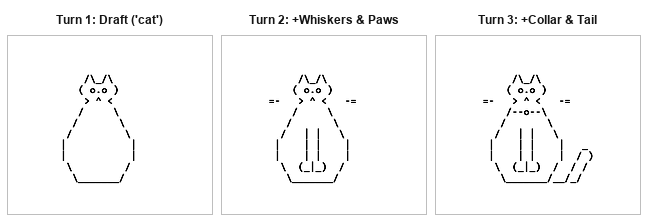
\includegraphics[width=0.94\linewidth]{figures/fig2_agentic_turns.png}
  \vspace{-2pt}
  \caption{\textbf{P2 Agentic Self-Perception Progression (Target: \texttt{cat}, Model: \texttt{gemini-3.1-flash-lite}).} Turn 1 drafts the head and torso silhouette. Inspecting the rendered PNG in Turn 2 guides localized \texttt{patch\_edit} calls for symmetric whiskers and seated front paws. Turn 3 adds a bell collar and curled tail.}
  \label{fig:agentic_turns}
\end{figure}

\begin{figure}[!t]
  \centering
  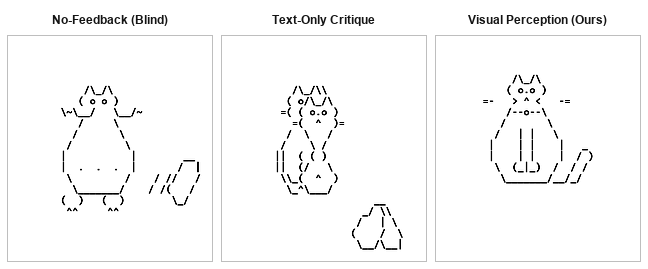
\includegraphics[width=0.94\linewidth]{figures/fig3_feedback_ablation.png}
  \vspace{-2pt}
  \caption{\textbf{P2 Feedback Mode Ablation on \texttt{cat}.} Left: \texttt{no\_feedback} (blind) overwrites the nose and places floating disconnected feet/tail. Center: \texttt{text\_only} critique misaligns row offsets, superimposing a second face over the first. Right: \texttt{visual} perception (ours) grounds every edit accurately.}
  \label{fig:ablation}
\end{figure}

\subsection{P2: Agentic Synthesis and Feedback Ablation}
Figure~\ref{fig:agentic_turns} illustrates the 3-turn agentic progression on \texttt{cat} using \texttt{gemini-3.1-flash-lite}. Even on the lightweight model, decomposing generation into $\text{draft} \to \text{render} \to \text{perceive} \to \text{revise}$ yields a clean, high-entropy drawing ($H = 3.14$ bits, 13 distinct chars, $\rho = 0.056$, coverage $= 0.165$). As shown in the Figure~\ref{fig:ablation} ablation, removing the rendered PNG causes severe spatial degradation: \texttt{no\_feedback} ($\rho = 0.058, H = 2.89$) hallucinates disconnected limbs to the right of the body, while \texttt{text\_only} ($\rho = 0.065, H = 2.92$) miscalculates row indices and stamps a duplicate face over the chest. Pairing the rendered PNG with the 2-digit coordinate ruler in \texttt{visual} mode eliminates both failure modes.

\subsection{P3: CLIP Evaluation and Judge Calibration}
Evaluating rendered drawings with local CLIP ViT-B/32 against text prompts (\texttt{"an ASCII art drawing of a \{category\}"}) confirms positive control gaps ($\Delta{\uparrow}$): the P2 \texttt{cat} achieves $S_{\text{real}} = 0.3251$ vs. $0.2737$ (\emph{scramble-cells}) and $0.2758$ (\emph{scramble-ink}), yielding $\Delta = +0.0493$; the P5 \texttt{bear} achieves $S_{\text{real}} = 0.2981$ vs. $0.2707$ scrambled ($\Delta = +0.0274$); and P1 procedural \texttt{horse} (\texttt{effort=low}) achieves $0.3213$ vs. $0.3088$ ($\Delta = +0.0124$). Crucially, on the truncated \texttt{effort=None} procedural \texttt{horse} where leaked plan prose spelled \texttt{"horse"} (\texttt{spells\_name=True}), CLIP yields $S_{\text{real}} = 0.1893$ vs. $0.2451$ scrambled ($\Delta = -0.0558 < 0$), proving that $\Delta$ penalizes text leakage. In our dual VLM judge test (\texttt{run\_judge\_text\_vs\_image.py}), the rendered P2 \texttt{cat} bitmap is identified as \texttt{"cat"} and rated $5/5$ vs. $1/5$ scrambled ($\Delta_{\text{judge}} = +4.0$).

\subsection{Unified Downstream Extensions (P4, P5, P6)}
To ensure strict experimental continuity, both our conversational editing (P4) and keyframe animation (P6) experiments take the \textbf{exact Turn 3 \texttt{cat} canvas synthesized by our P2 agentic loop} (Figure~\ref{fig:agentic_turns}, right) as their starting base drawing:
\begin{itemize}
  \item \textbf{P4: Conversational Editing (Figure~\ref{fig:extensions}a).} Given the P2 \texttt{cat} canvas and the instruction \emph{``Add a pointy party hat with a star on top of the head''}, the agent inspects the rendered image and 2-digit ruler and issues a single \texttt{patch\_edit} at rows 0--2, columns 18--22 (modifying only 8 cells directly above the ears \texttt{/\_/\textbackslash} at row 3 while leaving rows 3--23 completely untouched; $\rho: 0.056 \to 0.0625$, 14 distinct chars).
  \item \textbf{P5: Semantic Image-to-ASCII (Figure~\ref{fig:extensions}b).} Given a $320 \times 320$ shaded RGB illustration of a seated \texttt{bear} on a sky-and-foliage background (\texttt{runs/p5\_image2ascii/input\_photo.png}), the VLM suppresses background clutter and photometric gradients to extract a clean $24 \times 48$ structural contour ($\rho = 0.125$, coverage $= 0.391$, $H = 3.04$ bits, 11 distinct chars).
  \item \textbf{P6: Delta-Patched Keyframe Animation (Figure~\ref{fig:extensions}c).} Regenerating a full $24 \times 48$ grid per frame causes body drift and limb mutation. Instead, \texttt{p6\_animate.py} initializes each frame $t$ from $\text{AsciiCanvas}(\text{base}=\text{frame}_{t-1})$ and applies only localized \texttt{patch\_edit} deltas. Starting from the P2 \texttt{cat}, the head, whiskers, collar, torso, and paws remain 100\% invariant across frames while the eyes blink (\texttt{o.o} $\to$ \texttt{-.-} $\to$ \texttt{\textasciicircum.\textasciicircum}) and the tail wags.
\end{itemize}

\begin{figure}[!t]
  \centering
  \begin{subfigure}{0.54\linewidth}
    \centering
    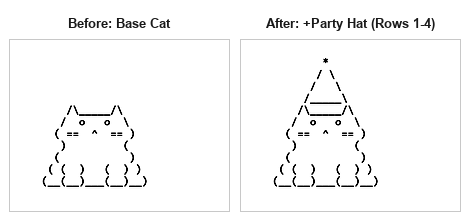
\includegraphics[width=\linewidth]{figures/fig4_conversational_edit.png}
    \caption{\textbf{P4 Edit:} +Party hat on P2 \texttt{cat}.}
  \end{subfigure}\hfill
  \begin{subfigure}{0.40\linewidth}
    \centering
    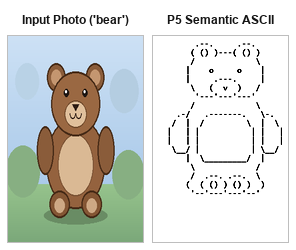
\includegraphics[width=\linewidth]{figures/fig6_image2ascii.png}
    \caption{\textbf{P5 Photo $\to$ ASCII} (\texttt{bear}).}
  \end{subfigure}
  \vspace{1pt}
  \begin{subfigure}{0.95\linewidth}
    \centering
    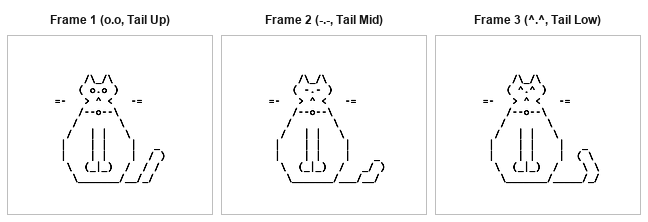
\includegraphics[width=\linewidth]{figures/fig5_animation_strip.png}
    \caption{\textbf{P6 Delta-Patched Animation:} Blinking eyes and wagging tail on the P2 \texttt{cat} with 100\% invariant body and limbs.}
  \end{subfigure}
  \vspace{-2pt}
  \caption{\textbf{Downstream Extensions (P4, P5, P6).} P4 and P6 operate directly on the P2 Turn 3 \texttt{cat} canvas; P5 converts an RGB image of a \texttt{bear} into semantic ASCII contours.}
  \label{fig:extensions}
\end{figure}

% =========================================================
\section{Discussion and Conclusion}
% =========================================================

\textbf{Comparison to SketchAgent and VideoSketcher.}
Whereas SketchAgent~\cite{vinker2025sketchagent} emits continuous parametric B\'{e}zier strokes on a vector canvas, ASCIIgent operates over a \emph{discrete character grid} via batched spatial primitives (\texttt{patch\_edit}, \texttt{draw\_line}, \texttt{shade\_density}) paired with a 2-digit coordinate ruler. In VideoSketcher~\cite{ren2025videosketcher}, an LLM decomposes a drawing plan into sequential strokes that a video diffusion model animates into pen-drawing footage. Because continuous diffusion does not apply to discrete text cells, ASCIIgent realizes dynamic synthesis in two discrete ways: (1) \textbf{procedural turn playback}, replaying the logged action sequence step-by-step (\texttt{progression.gif}), and (2) \textbf{delta-patched keyframe animation} (P6), where autoregressive visual conditioning and localized \texttt{patch\_edit} operations enforce frame-to-frame body invariance.

\textbf{Limitations and Future Work.}
Free-tier API rate limits constrain sample counts per cell, and VLM coordinate grounding still benefits from explicit 2-digit row/column rulers alongside rendered bitmaps. Future work includes expanding evaluations across additional open-weights and proprietary VLMs, calibrating the scrambled control gap $\Delta$ against human perceptual studies, and incorporating tree search over candidate discrete edits.

\textbf{Conclusion.}
ASCIIgent demonstrates that while monolithic autoregressive generation is vulnerable to scanline drift, glyph collapse, and plan-truncation leakage, coupling a discrete spatial action vocabulary with active visual perception enables self-correcting ASCII synthesis, surgical conversational editing, semantic image-to-ASCII abstraction, and coherent keyframe animation.

{\scriptsize
\bibliographystyle{ieeetr}
\bibliography{references}
}

\end{document}
